\documentclass[letterpaper]{article} % DO NOT CHANGE THIS
\usepackage{aaai24}  % DO NOT CHANGE THIS
\usepackage{times}  % DO NOT CHANGE THIS
\usepackage{helvet}  % DO NOT CHANGE THIS
\usepackage{courier}  % DO NOT CHANGE THIS
\usepackage[hyphens]{url}  % DO NOT CHANGE THIS
\usepackage{graphicx} % DO NOT CHANGE THIS
\urlstyle{rm} % DO NOT CHANGE THIS
\def\UrlFont{\rm}  % DO NOT CHANGE THIS
\usepackage{natbib}  % DO NOT CHANGE THIS AND DO NOT ADD ANY OPTIONS TO IT
\usepackage{caption} % DO NOT CHANGE THIS AND DO NOT ADD ANY OPTIONS TO IT
\frenchspacing  % DO NOT CHANGE THIS
\setlength{\pdfpagewidth}{8.5in}  % DO NOT CHANGE THIS
\setlength{\pdfpageheight}{11in}  % DO NOT CHANGE THIS
\usepackage{algorithm}
\usepackage{algorithmic}
\usepackage{newfloat}
\usepackage{listings}
\DeclareCaptionStyle{ruled}{labelfont=normalfont,labelsep=colon,strut=off} % DO NOT CHANGE THIS
\lstset{%
	basicstyle={\footnotesize\ttfamily},% footnotesize acceptable for monospace
	numbers=left,numberstyle=\footnotesize,xleftmargin=2em,% show line numbers, remove this entire line if you don't want the numbers.
	aboveskip=0pt,belowskip=0pt,%
	showstringspaces=false,tabsize=2,breaklines=true}
\floatstyle{ruled}
\newfloat{listing}{tb}{lst}{}
\floatname{listing}{Listing}
\pdfinfo{
/TemplateVersion (2024.1)
}

\setcounter{secnumdepth}{0} %May be changed to 1 or 2 if section numbers are desired.

\usepackage{bibentry}

\title{CS-GY 6953 Project 1}
\author{Matthew So\textsuperscript{\rm 1}}
\affiliations{\textsuperscript{\rm 1}Tandon School of Engineering\\New York University\\m.so@nyu.edu}

\begin{document}

\maketitle

\begin{abstract}
We aim to achieve the highest possible accuracy on an unknown, custom test set.  The task is to train a ResNet-type model (or other convolutional neural network) with under 5M parameters on the CIFAR-10 dataset.  In this project, we use an implementation of Wide Residual Networks \cite{zagoruyko2017wideresidualnetworks}, which achieved state-of-the-art (SOTA) performance on CIFAR-10 in 2017.  We reproduce their findings and only add minor data augmentation modifications to increase our performance on the unknown test set, leading to an accuracy of 84.68.

Project code can be found at this link - \url{https://github.com/ms15032/project-1}.
\end{abstract}

\section{Introduction}

Traditional ResNets are usually networks with many layers.  The purpose of the residual connection was to ensure gradients don't vanish in networks with hundreds or even thousands of layers.  In \cite{zagoruyko2017wideresidualnetworks}, the authors show that competitive performance can be achieved by using "wide" networks as opposed to "deep" networks.  In this case, "width" is proportional to the number of convolutional filters used in each block.  Each block still contains a residual connection, so these networks are called WRNs (Wide Residual Networks).

This network architecture was chosen because of its high performance on the CIFAR-10 dataset.  In 2017, this paper achieved SOTA performance on CIFAR-10 compared to other ResNets.  Today's SOTA results only achieve accuracy improvements in the single digits, and almost always involve transformer architectures or pretraining on other datasets, all of which is not in the scope of this project.  It is also highly configurable (mainly, the depth and width parameters $d$ and $k$), so the number of parameters can be adjusted to fit the requirement of 5M parameters.

\section{Methodology}

Our implementation was a faithful reproduction of the authors' original implementation.  Our model was written as a PyTorch module and trained in a Kaggle notebook with an Nvidia P100 GPU for 200 epochs.  The Cross Entropy loss was used with a Stochastic Gradient Descent optimizer with a learning rate of 0.1, momentum of 0.9, and weight decay of 0.0005, all of which are clearly stated by the original authors.  A learning rate scheduler started at 0.1 and decreased by 0.2 times at epochs 60, 120, and 160.  This is to allow the model to quickly find minima, then refine that guess by using a smaller learning rate after a certain period.  This is clearly visible in the training curves (Fig. \ref{fig1}, \ref{fig2}, \ref{fig3}, \ref{fig4}) - loss makes a marked decrease and accuracy makes a marked increase at epochs 60 and 120, with a smaller difference at epoch 160.

\section{Results}

\begin{table}[t]
\centering
\begin{tabular}{|c|c|c|c|c|c|c|}
    \hline
    $d$ & $k$ & Params & Transforms & Train & Test & Custom \\
    \hline
    40 & 2 & 2.2M & Flip & 99.75 & 95.25 & 83.52 \\
    & & & Crop & & & \\
    22 & 4 & 4.3M & Flip & 99.87 & 95.79 & 84.68 \\
    & & & Crop & & & \\
    & & & Color & & & \\
    22 & 4 & 4.3M & Flip & 98.99 & 95.34 & 84.58 \\
    & & & Crop & & & \\
    & & & Color & & & \\
    & & & Affine & & & \\
    \hline
\end{tabular}
\caption{Train set, test set, and custom test set accuracies for 3 model and training variants.}
\label{table1}
\end{table}

Our first run used a network with depth 40 and width 2, totaling 2.2M parameters.  The original authors did not use many data augmentations, only a random horizontal flip and random crop of 32x32.  Since the original images are also 32x32, a padding of 4 was used with the "reflect" padding mode applied.  The images were then rescaled to values with a mean of (0.491, 0.482, 0.447) and standard deviation of (0.247, 0.244, 0.262), which were also defined in the original paper.  We were able to reproduce the results stated in the paper, achieving a train accuracy of 99.75 and test accuracy of 95.25 (Fig. \ref{fig1}, \ref{fig2}).  We observed a sharp decrease in accuracy on the custom test set of 83.52, so aimed to achieve further generalization of the model.

Our second run used a larger model with $d=22$ and $k=4$.  This model is not tested by the original authors, but was a suitable combination to increase the model parameters as close as possible to the limit of 5M.  The authors had observed higher performance with higher widths, so we increased the width to 4 and decreased the depth until the number of parameters reached less than 5M (in this case, 4.3M).  Attempting to increase generalization capabilities, we also added a color data augmentation, with brightness, color, and saturation randomly perturbed by 20\%.  The model reached its maximum accuracy much quicker, presumably because of its larger size.  We achieved a higher custom test set accuracy of 84.68 (Fig. \ref{fig3}, \ref{fig4}).

Lastly, we attempted to add additional data augmentations to further increase generalization capabilities.  We added a random affine transformation, which randomly applies a random rotation up to a maximum of 15 degrees, a random vertical or horizontal translation of 20\%, a random zoom-in or out by 20\%, and a random shear to a maximum of 15 degrees.  This made the dataset much harder for the model to learn, though it still reached a train accuracy of 98.99 and a test accuracy of 95.34.  This exhibited very slightly less overfitting, but the custom test accuracy was still slightly lower at 84.58.

The best performing model, a WRN with depth 22 and width 4 and totaling 4.3M parameters, achieved a custom test set accuracy of 84.68.  The transforms used were horizontal flip, crop, and color perturbations.  The loss, optimizer, and learning rate schedule were not changed from the original implementation defined in the paper.

Since it wasn't clear what data is contained in the custom test set, and accuracy on the CIFAR-10 test set was already quite high for models within this scope, we did not experiment further.  Based on our 3 runs, we did not foresee any benefit from additional model parameter changes or data augmentations.

\begin{figure}[t]
\centering
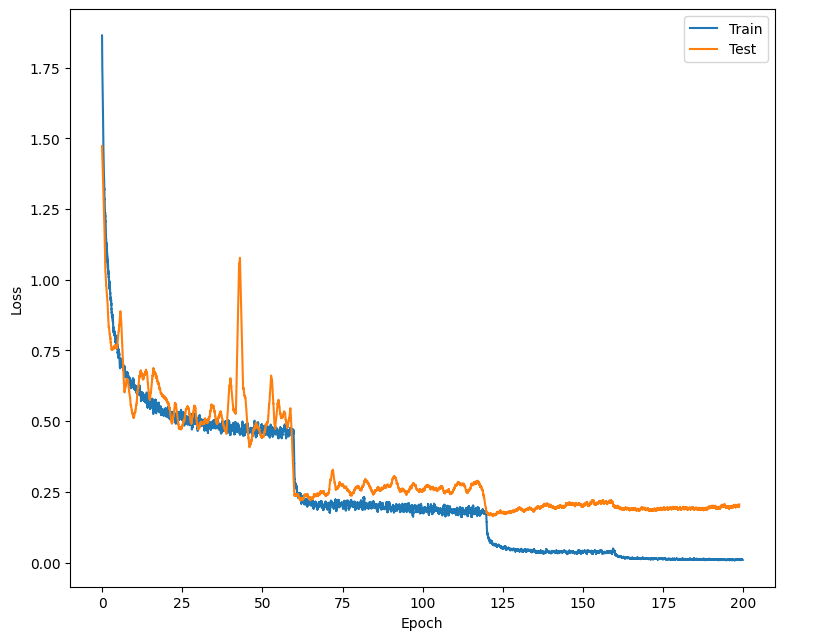
\includegraphics[width=0.95\columnwidth]{loss_2M.png}
\caption{Train and test loss over 200 epochs for the 2.2M model with flip and crop data augmentations.}
\label{fig1}
\end{figure}

\begin{figure}[t]
\centering
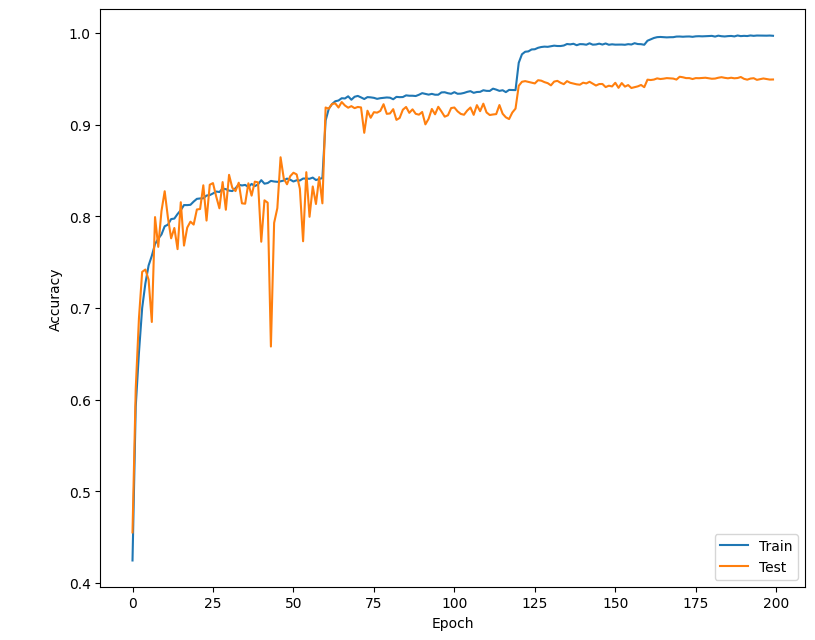
\includegraphics[width=0.95\columnwidth]{accuracy_2M.png}
\caption{Train and test accuracy over 200 epochs for the 2.2M model with flip and crop data augmentations.}
\label{fig2}
\end{figure}

\begin{figure}[t]
\centering
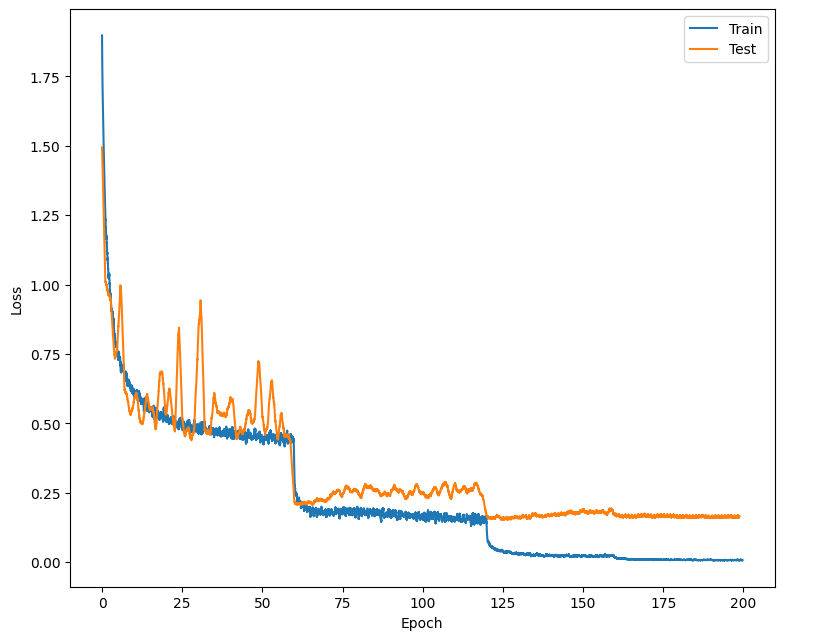
\includegraphics[width=0.95\columnwidth]{loss_4M.png}
\caption{Train and test loss over 200 epochs for the 4.3M model with flip, crop, and color data augmentations.}
\label{fig3}
\end{figure}

\begin{figure}[t]
\centering
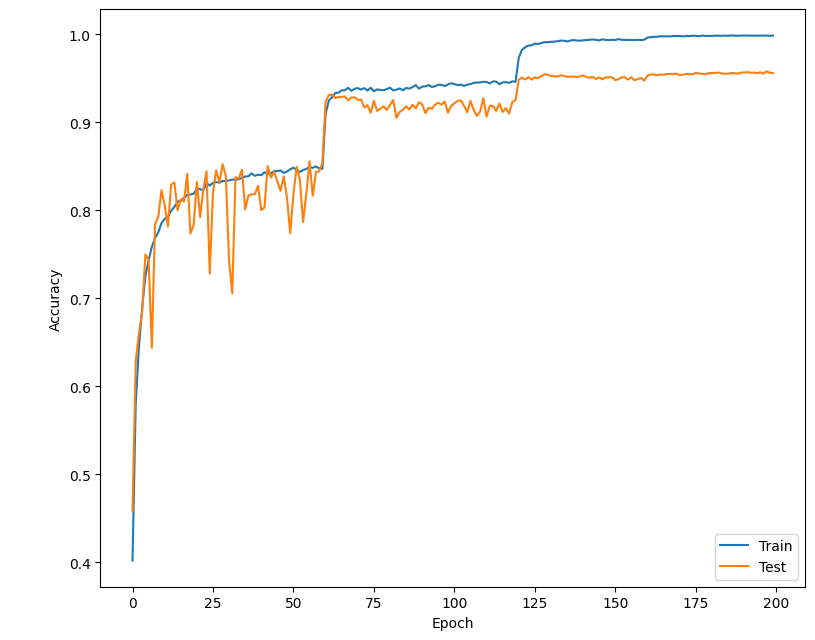
\includegraphics[width=0.95\columnwidth]{accuracy_4M.png}
\caption{Train and test accuracy over 200 epochs for the 4.3M model with flip, crop, and color data augmentations.}
\label{fig4}
\end{figure}

\bibliography{aaai24}

\end{document}